\subsubsection{Webpack}
Webpack - это инструмент для сборки модулей. Он может анализировать приложение, создавать его граф зависимостей и собирать приложение в виде бандлов (совокупностей программных данных, объединённых по какому-либо признаку), на которые приложение будет ссылаться при выполнении~\cite{Webpack}.

Обычно при разработке приложения, не важно, frontend или backend, код разделяется на несколько частей (модулей), обеспечивающих специфичные методы обработки данных. Но это может повлечь множество проблем при разработке и выполнении программы, таких как, например, разработчик может забыть подключить какие-либо скрипт или расположить их в неправильном порядке. Например, если вызывать скрипт, в котором используется какой-либо фреймворк до того, как он был загружен, приложение будет выполняться неправильно.

Webpack позволяет избежать подобные ситуации и берёт сборку приложения на себя.

Сборка приложения включает в себя создание бандлов приложения, подключение необходимых зависимостей, преобразование кода к минифицированному и другие этапы. Все эти этапы разработчик может указать в отдельном файле конфигурации и использовать при сборке.

В общем виде, работа Webpack показана на рисунке~\ref{img:webpack}

\begin{figure}[H]
  \centering
  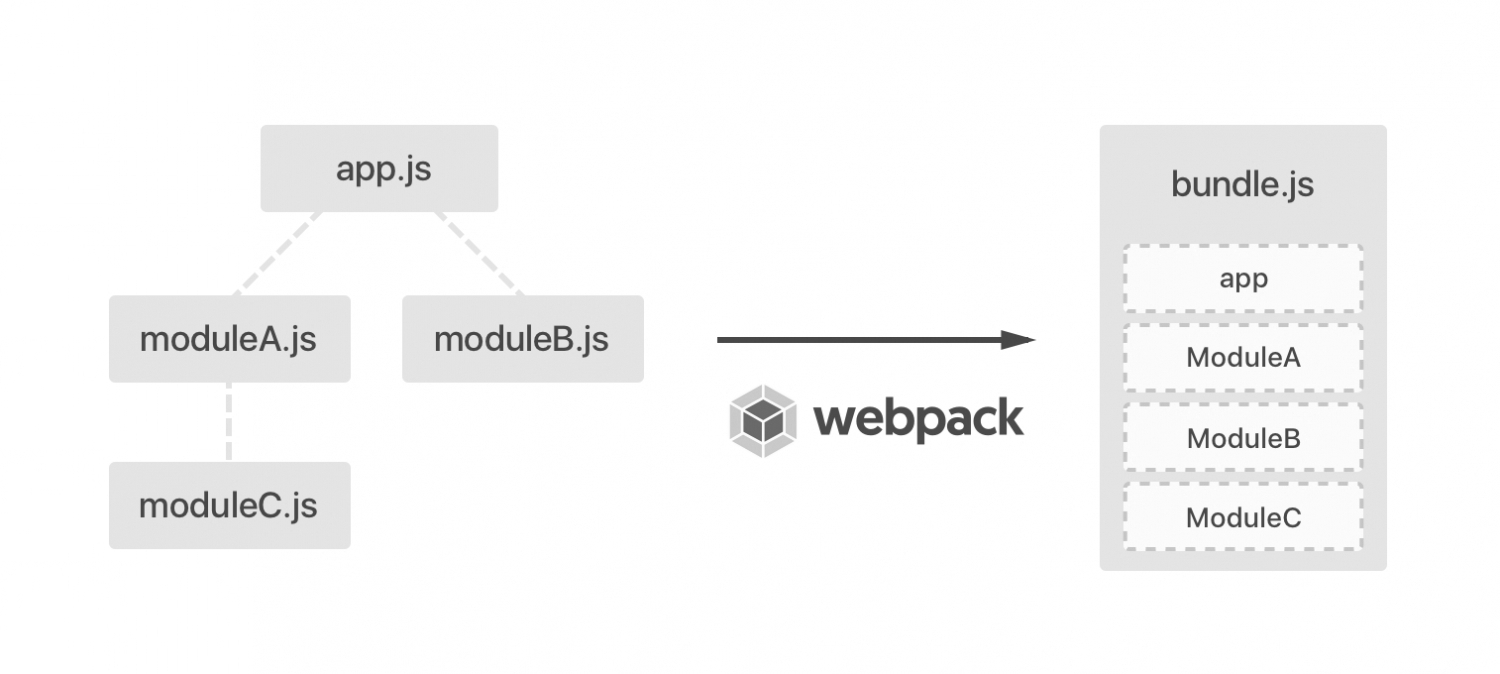
\includegraphics[width=0.95\textwidth]{assets/images/theoretical/webpack.jpg}
  \caption{Работа Webpack}
  \label{img:webpack}
\end{figure}